\documentclass{article}
\usepackage[a4paper,width=190mm,top=25mm,bottom=25mm]{geometry}
\usepackage[utf8]{inputenc}
\usepackage{listings} % to write code of programming
\usepackage{verbatim}
\usepackage{lineno}
\usepackage{hyperref} 
\hypersetup{
	citecolor=blue,
	colorlinks=true,
	linkcolor=blue,
	filecolor=magenta,      
	urlcolor=blue,
	pdftitle={ADP},
	pdfpagemode=FullScreen,
}
\usepackage{amsmath}
\usepackage{amssymb}
\usepackage{amsthm}
\usepackage{bm}
\usepackage{svg}
\usepackage{cleveref}
\usepackage[fleqn,tbtags]{mathtools}
\usepackage{amsfonts}
%\usepackage{standalone}
\usepackage{environ}
\usepackage{slashed}
\usepackage{textcomp}
%\usepackage{subfig}
\usepackage{subfigure}
\usepackage{caption}
\usepackage{soul}
\usepackage{xstring}
\usepackage{glossaries}
\usepackage{comment}
\usepackage{physics}
\usepackage{xcolor}
\definecolor{codegreen}{rgb}{0,0.6,0}
\definecolor{codegray}{rgb}{0.5,0.5,0.5}
\definecolor{codepurple}{rgb}{0.58,0,0.82}
\definecolor{backcolour}{rgb}{0.95,0.95,0.95}
\usepackage{enumitem}
\usepackage{graphicx}



%\makeglossaries


\title{C++ Script to convert potential data file of LAMMPS format to SOLERA format}

\author{\small José Manuel Recio-López (PhD Student) / Advisors: Pilar Ariza (Full Professor) and Miguel Molinos (PhD) \\ WORKING NOTES, NOT DISTRIBUTION}%Documentation for SOLERA}

\date{$23^{rd}$ Jul 2024}

\begin{document}

\maketitle

%%%%%%%%%%%%%%%%%%%%%%%%%%%%%%%%%%%%%%%%%%%%%%%%%%%%%%%%%%%%%%%%%%%%%%%%%%%%%%%%%%%%%%
\vspace{0.5cm}
\hrule
\vspace{0.5cm}
%%%%%%%%%%%%%%%%%%%%%%%%%%%%%%%%%%%%%%%%%%%%%%%%%%%%%%%%%%%%%%%%%%%%%%%%%%%%%%%%%%%%%%

\section{The Angular-Dependent Potential (ADP) file of LAMMPS}

The potential data file is obtained of the Interatomic Potentials Repository (IPR) of the National Institute of Standards and Technology (NIST) of the U.S.A. (\href{https://www.ctcms.nist.gov/potentials}{www.ctcms.nist.gov/potentials}). 

The Angular-Dependent Potential (ADP) was developed by Mishin et al. \cite{MisMehPap05,ApoMis11} and it is an extension of the Embedded Atom Method (EAM) formalism, suggested by Daw and Baskes \cite{DawBas84,FoiBasDaw86}, adding angular dependent dipole and quadrupole terms, which represent the dipole and quadruple distortions of the local atomic environment by introducing angular forces.

ADP files, in the potentials directory of the LAMMPS code,  have an \textit{``.adp''} suffix and a DYNAMO \textit{setfl format}. The DYNAMO \textit{setfl format} was designed for an EAM potential. A DYNAMO \textit{setfl format} extended for ADP is formatted of the same way that the standard \textit{setfl format} for an EAM potential with additional tabulated functions \textit{u} and \textit{w} added to the file after the tabulated pair potentials. Let's see how is the format of this file: 

\begin{enumerate}
	\item The header is constituted by 5 lines:
	
	\begin{itemize}
		\item The lines 1, 2 and 3 are comments about the potential. They can be ignored.
		\item The format of the line 4 is: ``$N$ $E_1$ $E_2$ $...$ $E_{N}$'', where $N$ is the number of elements which are involved in the potential and $E_i$ the chemical symbol of the element $i$, with $i=1,2,...,N$.  
		\item The format of the line 5 is: ``$N_{\rho}$ $d_{\rho}$ $N_r$ $d_r$ $r_{c}$'', where $N_{\rho}$ is the number of values of the atomic electron density $\rho$ to evaluate the embedding function $F(\rho)$, $d_{\rho}$ is the increment in the values of the atomic electron density $\rho$, $N_r$ is the number of values of the distance $r$ between the atomic pair to evaluate the atomic electron density $\rho$, $d_r$ is the increment in the values of $r$, and $r_{c}$ is the value of cutoff distance for the pair interaction. 
	\end{itemize}
	\item After the header lines, $N$ sections are listed, one for each element, each with the following format:
	
	\begin{itemize}
		\item First line: ``$Z$ $M$ $a$ $lattice$'', where $Z$ is the atomic number of the element, $M$ is its atomic mass, $a$ is the lattice constant, and $lattice$ is the lattice type.
		\item Block of $N_\rho$ values corresponding to the embedding function $F(\rho)$.
		\item Block of $N_r$ values corresponding to the atomic electron density $\rho(r)$.
	\end{itemize}
	\item Following the $N$ data sections above, values with a scaling by $r$ for each pair potential function $\phi_{(i,j)}(r)$, namely, as $r\cdot\phi_{(i,j)}(r)$ (in units of eV-Angstroms), are listed for all ($i,j$)
	element pairs, since they are for atom pairs. Due to these interactions are symmetric ($\phi_{(i,j)}(r)=\phi_{(j,i)}(r)$) only arrays with $i\leq j$ are listed, in the following order: $(i,j)=(1,1),(1,2),(2,2),(1,3),(2,3),(3,3),(1,4),...,(1,N),(2,N),...,(N,N)$. In total, there are $N(N+1)/2$ arrays (combinations with repetition of $N$ elements grouped by pairs). Therefore, the format of this data section is:
	\begin{itemize}
		\item Block of $N_r$ values corresponding to the scaled pair potential function $r\phi_{(1,1)}(r)$.
		\item ...
		\item Block of $N_r$ values corresponding to the scaled pair potential function $r\phi_{(N,N)}(r)$.
	\end{itemize}
	\item Following the $N_r N(N+1)/2$ data section above, corresponding to each scaled pair potential function, are listed the functions $u_{(i,j)}(r)$ in the same format and under the same assumptions of symmetry. Thus, the next lines have this format:
	\begin{itemize}
		\item Block of $N_r$ values corresponding to the function $u_{(1,1)}(r)$.
		\item ...
		\item Block of $N_r$ values corresponding to the function $u_{(N,N)}(r)$.
	\end{itemize}
	\item Finally, behind the section of $N_r N(N+1)/2$ data corresponding to the functions $u_{(i,j)}(r)$, the functions $w_{(i,j)}(r)$ are listed in the same format and under the same assumptions of symmmetry that the functions $u_{(i,j)}(r)$. Therefore, the format of this data section is:
	\begin{itemize}
		\item Block of $N_r$ values corresponding to the function $w_{(1,1)}(r)$.
		\item ...
		\item Block of $N_r$ values corresponding to the function $w_{(N,N)}(r)$.
	\end{itemize}
\end{enumerate}

Note that only the pair potential functions are scaled by $r$. Information taken from \href{https://docs.lammps.org/pair_adp.html}{\textit{pair\_style adp}} command of LAMMPS.


\section{Adapting of the ADP file of LAMMPS format to SOLERA format}
The script \textit{adp.cpp} has been created for the adapting of the ADP file, which is named as \textit{filename.adp}, to SOLERA format. The input is the \textit{filename.adp} file and the outputs are the following files:

\subsection{Cubic spline}
Once the data of the functions are collected, a polynomial interpolation is performed for each function through cubic spline to have a piecewise analytical function with continuous second derivative.

If we have a function defined through $n$ points $x_i$, with $i=0,1,2,...,n-1$, we will obtain $n-1$ segments $S_j(x)$, with $j=0,1,2,...,n-2$, of the cubic spline which approximates to the function with the next way:

\begin{equation}
	S_j(x)=a_j+b_j(x-x_j)+c_j(x-x_j)^2+d_j(x-x_j)^3
\end{equation}

The first derivative of the spline is
\begin{equation}
	S'_j(x)=b_j+2c_j(x-x_j)+3d_j(x-x_j)^2=db_j+dc_j(x-x_j)+dd_j(x-x_j)^2
\end{equation}
where $db_j=b_j$, $dc_j=2c_j$, y $dd_j=3d_j$ are the coefficients of the first derivative of the spline, and the second derivative of the spline is
\begin{equation}
	S''_j(x)=2c_j+6d_j(x-x_j)=ddc_j+ddd_j(x-x_j)
\end{equation}
where $ddc_j=2c_j$, y $ddd_j=6d_j$ are the coefficients of the second derivative of the spline.

To determine the coefficients $a_j,b_j,c_j$ and $d_j$ is applied the algorithm for natural cubic splines in the chapter 3 of the reference \cite{BurFai11}. 

The calculation of the value of the spline in a point $x$ is determined applying the Horner's iterative method which consists in expressing the polynomial in this way:

\begin{equation}
	S_j(x)=a_j+\left\{b_j+\left[c_j+d_j(x-x_j)\right](x-x_j)\right\}(x-x_j)
\end{equation} 


The algorithm to construct the natural cubic spline interpolant $S(x)$ for a function $f(x)$ (see chapter 3 in \cite{BurFai11}), defined at the points $x_0 < x_1 < ... < x_n$, satisfying $S''(x_0) = S''(x_n) = 0$ is the following:\\

(Note: $S(x) = S_j(x) = a_j + b_j(x-x_j) + c_j(x-x_j)^2 + d_j(x -x_j)^3$ for $x_j \le x \le x_{j+1}).$\\

INPUT: $n; x_0, x_1, ... , x_n; a_0 = f(x_0), a_1 = f (x_1), ... , a_n = f (x_n).$\\

ALGORITHM:

\textbf{Step 1} For $i = 0, 1, ... , n-1$ set $h_i = x_{i+1}-x_i$.

\textbf{Step 2} For $i = 0, 1, ... , n-1$ set $\alpha_i = 3h_i(a_{i+1}-a_i)-3h_{i-1}(a_i-a_{i-1})$.

(Steps 3, 4, 5, and part of Step 6 solve a tridiagonal linear system).

\textbf{Step 3} Set $l_0 = 1$; $\mu_0 = 0$; $z_0 = 0$.

\textbf{Step 4} For $i = 1, 2, . . . , n-1$ set $l_i = 2(x_{i+1}-x_{i-1})-h_{i-1}\mu_{i-1}$; $\mu_i = h_i/l_i$; $z_i = (\alpha_i-h_{i-1}z_{i-1})/l_i$.

\textbf{Step 5} Set $l_n = 1$; $z_n = 0$; $c_n = 0$.

\textbf{Step 6}  For $j = n-1, n-2, ... , 0$ set $c_j = z_j- \mu_jc_{j+1}$;
$b_j = (a_{j+1}-a_j)/h_j-h_j(c_{j+1} + 2c_j)/3$;
$d_j = (c_{j+1}-c_j)/(3h_j)$.\\

OUTPUT: $a_j,b_j,c_j,d_j$ for $j=0,1,...,n-1$.



\subsection{Files}

\begin{itemize}
	\item \textit{adp*.dat}: files with the SOLERA format. There are $N(N+1)/2$ files. Thus, for the Al-Cu system we have the three followings files: \textit{adpAl.dat}, \textit{adpAlCu.dat}, and \textit{adpCu.dat}. 
	
	The single element files (\textit{adpMg.dat} and \textit{adpH.dat} for the case of the Mg-H system or \textit{adpAl.dat} and \textit{adpCu.dat} for the case of the Al-Cu system) have a header with three values and five blocks of data corresponding to the five functions $\rho(r),F(\bar{\rho}),\phi(r),u(r)$ and $w(r)$, in this order. The header is the first row: the first value in the first row is the atomic mass $M$ of the element, the second value is a factor, and the third value is the cutoff radius $r_c$. Next, each data block contains a first line with two values followed by a data matrix. In the first line of the each data block, the first value is the number of segments $n-1$ of the spline and the second value is the increment in the independent variable considered in the function. The data matrix in each block contains the spline data and its first and second derivatives formed by $n-1$ lines and nine columns. The first four columns contain the $n-1$ sets of coefficients of the segments of the spline $a_j,b_j,c_j$ and $d_j$, the following three columns contain the $n-1$ sets of coefficients of the segments of the first derivative of the spline $db_j,dc_j$ and $d_j$, and the following two columns contain the $n-1$ sets of coefficients of the segments of the second derivative of the spline $ddc_j$ and $ddd_j$, in this order, for $j=0,1,2,...,n-2$.
	
	The cross element files (\textit{adpMgH.dat} for the case of the Mg-H system or \textit{adpAlCu.dat} for the case of the Al-Cu system) have a header and three blocks of data corresponding to the three functions $\phi(r),u(r)$ and $w(r)$, in this order. The header is the first row which only contains one value corresponding to the cutoff radius $r_c$. Next, each data block contains a first line with two values followed by a data matrix at the same way that the single element files, but three blocks only appears: the first block is for the function $\phi(r)$, the second block is for the function $u(r)$ and the third block is for the function $w(r)$.
	
	\item \textit{F.dat}: file with data of the embedding function $F$ for each element as a function of the host electronic density $\bar{\rho}$. The first column contains the index of the point, the second column contains the data array with the host electronic density $\bar{\rho}$, and the following columns contain the data array of the embedding function $F(\bar{\rho})$ for each element.  
	
	\item \textit{rho.dat}: file with the data of the electronic density function $\rho$ for each element. The first column contains the index of the point, the second column contains the data array with the interatomic distance $r$, and the following columns contain the data array of the electronic density function $\rho(r)$ for each element.  
	
	\item \textit{phi.dat}: file with the data of the pairs energy function $\phi$. The first column contains the index of the point, the second column contains the data array with the interatomic distance $r$, and the following columns contain the data array of the pairs energy function $\phi(r)$ for each element pair in this order: $(1,1),(1,2),(2,2),(1,3),(2,3),(3,3),(1,4),...,(1,N),$ $(2,N),...,(N,N)$.
	
	\item \textit{u.dat}: file with the data of the dipole function $u$. The first column contains the index of the point, the second column contains the data array with the interatomic distance $r$, and the following columns contain the data array of the function $u(r)$ for each element pair in the same order that the function $\phi$.
	
	\item \textit{w.dat}: file with the data of the quadrupole function $w$. The first column contains the index of the point, the second column contains the data array with the interatomic distance $r$, and the following columns contain the data array of the function $w(r)$ for each element pair in the same order that the function $\phi$.
\end{itemize}

At these files, the value 0 of the functions $\rho(r),\phi(r),u(r)$ y $w(r)$, corresponding to the cutoff distance $r_{c}$, is added to the data extracted from the ADP file whether it doesn't appears in this file, that is, the points $(r_c, 0)$ of each function. It can be verified the functions $\rho(r),\phi(r),u(r)$ y $w(r)$ take the value 0 when the distance is $r_c$.




\section{Case of the Mg-H system}

For the Mg-H system, the ADP file that we find in the IPR is called \textit{``Mg\_H.adp.alloy.txt''} and its format is the following:

%%%%%%%%%%%%%%%%%%%%%%%%%%%%%%%%%%%%%%%%%%%%%%%%%%%%%%%%%%%%%%%%%
%%%%%%%%%%%%%%%%%%%%%%%%%%%%%%%%%%%%%%%%%%%%%%%%%%%%%%%%%%%%%%%%%
%\begin{comment}
	\setlist[enumerate]{label*=\arabic*.}
	\begin{enumerate}
		\item Header:
		\lstdefinestyle{mystyle}{
			backgroundcolor=\color{backcolour},   
			commentstyle=\color{codegreen},
			keywordstyle=\color{black},
			numberstyle=\tiny\color{codegray},
			stringstyle=\color{codepurple},
			basicstyle=\ttfamily\scriptsize,
			breakatwhitespace=false,         
			breaklines=true,                 
			captionpos=b,                    
			keepspaces=true,                 
			numbers=left,                    
			numbersep=2pt,                  
			showspaces=false,                
			showstringspaces=false,
			showtabs=false,                  
			tabsize=1,
			xleftmargin=10pt,
			xrightmargin=5pt,
			fontadjust=true
		}
		\lstset{style=mystyle}
		%\lstinputlisting[language=Matlab,linerange={1-5},consecutivenumbers=false]{Mg_H.adp.alloy.txt}
		\item  Sections for the embedding function $F(\rho)$ and the atomic electron density $\rho(r)$ of the $N=2$ elements:
		
		
		\begin{enumerate}
			\item Section of the Mg (element 1):
			
			First line:
			%\lstinputlisting[language=Matlab,linerange={6},consecutivenumbers=false]{Mg_H.adp.alloy.txt}
			
			Block of $N_{\rho}=968$ values corresponding to the embedding function $F(\rho)$ for Mg:
			%\lstinputlisting[language=Matlab,linerange={7-9,972-974},consecutivenumbers=false,]{Mg_H.adp.alloy.txt}
			
			Block of $N_{r}=1195$ values corresponding to the atomic electron density $\rho(r)$ for Mg:
			%\lstinputlisting[language=Matlab,linerange={975-977,2167-2169},consecutivenumbers=false]{Mg_H.adp.alloy.txt}
			
			\item Section of the H (element 2):
			
			First line:
			%\lstinputlisting[language=Matlab,linerange={2170},consecutivenumbers=false]{Mg_H.adp.alloy.txt}
			
			Block of $N_{\rho}=968$ values corresponding to the embedding function $F(\rho)$ for H:
			%\lstinputlisting[language=Matlab,linerange={2171-2173,3136-3138},consecutivenumbers=false]{Mg_H.adp.alloy.txt}
			
			Block of $N_{r}=1195$ values corresponding to the atomic electron density $\rho(r)$ for H:
			%\lstinputlisting[language=Matlab,linerange={3139-3141,4331-4333},consecutivenumbers=false]{Mg_H.adp.alloy.txt}
		\end{enumerate}

		\item  Block of $N_rN(N+1)/2=3585$ values corresponding to the scaled pair potential functions $r\phi_{(i,j)}(r)$:
		\begin{enumerate}
			\item Block of $N_r=1195$ values corresponding to the scaled pair potential function $r\phi_{(Mg,Mg)}(r)$:
			%\lstinputlisting[language=Matlab,linerange={4334-4336,5526-5528},consecutivenumbers=false]{Mg_H.adp.alloy.txt}
			
			\item Block of $N_r=1195$ values corresponding to the scaled pair potential function $r\phi_{(Mg,H)}(r)$:
			%\lstinputlisting[language=Matlab,linerange={5529-5531,6721-6723},consecutivenumbers=false]{Mg_H.adp.alloy.txt}
			
			\item Block of $N_r=1195$ values corresponding to the scaled pair potential function $r\phi_{(H,H)}(r)$:
			%\lstinputlisting[language=Matlab,linerange={6724-6726,7916-7918},consecutivenumbers=false]{Mg_H.adp.alloy.txt}
		\end{enumerate}
		
		\item  Block of $N_rN(N+1)/2=3585$ values corresponding to the functions $u_{(i,j)}(r)$:
		\begin{enumerate}
			\item Block of $N_r=1195$ values corresponding to the function $u_{(Mg,Mg)}(r)$:
			%\lstinputlisting[language=Matlab,linerange={7919-7921,9111-9113},consecutivenumbers=false]{Mg_H.adp.alloy.txt}
			
			\item Block of $N_r=1195$ values corresponding to the function $u_{(Mg,H)}(r)$:
			%\lstinputlisting[language=Matlab,linerange={9114-9116,10306-10308},consecutivenumbers=false]{Mg_H.adp.alloy.txt}
			
			\item Block of $N_r=1195$ values corresponding to the function $u_{(H,H)}(r)$:
			%\lstinputlisting[language=Matlab,linerange={10309-10311,11501-11503},consecutivenumbers=false]{Mg_H.adp.alloy.txt}
		\end{enumerate}
		
		
		\item  Block of $N_rN(N+1)/2=3585$ values corresponding to the functions $w_{(i,j)}(r)$:
		\begin{enumerate}
			\item Block of $N_r=1195$ values corresponding to the function $w_{(Mg,Mg)}(r)$:
			%\lstinputlisting[language=Matlab,linerange={11504-11506,12696-12698},consecutivenumbers=false]{Mg_H.adp.alloy.txt}
			
			\item Block of $N_r=1195$ values corresponding to the function $w_{(Mg,H)}(r)$:
			%\lstinputlisting[language=Matlab,linerange={12699-12701,13891-13893},consecutivenumbers=false]{Mg_H.adp.alloy.txt}
			
			\item Block of $N_r=1195$ values corresponding to the function $w_{(H,H)}(r)$:
			%\lstinputlisting[language=Matlab,linerange={13894-13896,15086-15088},consecutivenumbers=false]{Mg_H.adp.alloy.txt}
		\end{enumerate}
	\end{enumerate}
%\end{comment}
%%%%%%%%%%%%%%%%%%%%%%%%%%%%%%%%%%%%%%%%%%%%%%%%%%%%%%%%%%%%%%%%%
%%%%%%%%%%%%%%%%%%%%%%%%%%%%%%%%%%%%%%%%%%%%%%%%%%%%%%%%%%%%%%%%%

Next, the output files for the Mg-H system created by the script \textit{adp.cpp} are represented.


\begin{figure}[h!]
	\centering
	%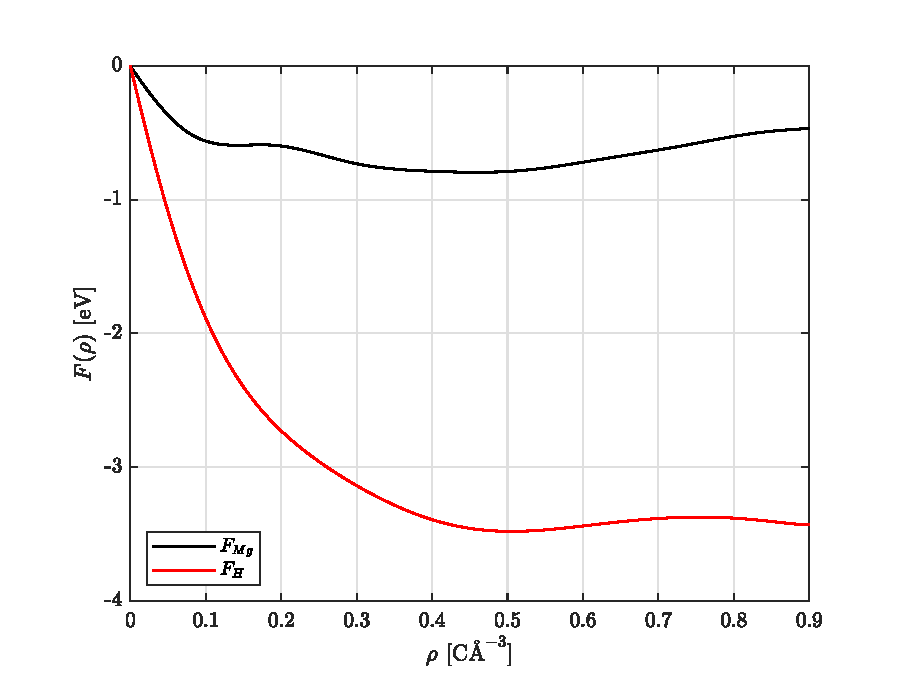
\includegraphics[width=\textwidth]{Figures/F_MgH.eps}
	\includegraphics[width=\textwidth]{Figures/Fig-Embeding-Energy.png}
\caption{Embedding function $F(\rho)$ for each element}
\end{figure}
\begin{figure}[h!]
	\centering
	%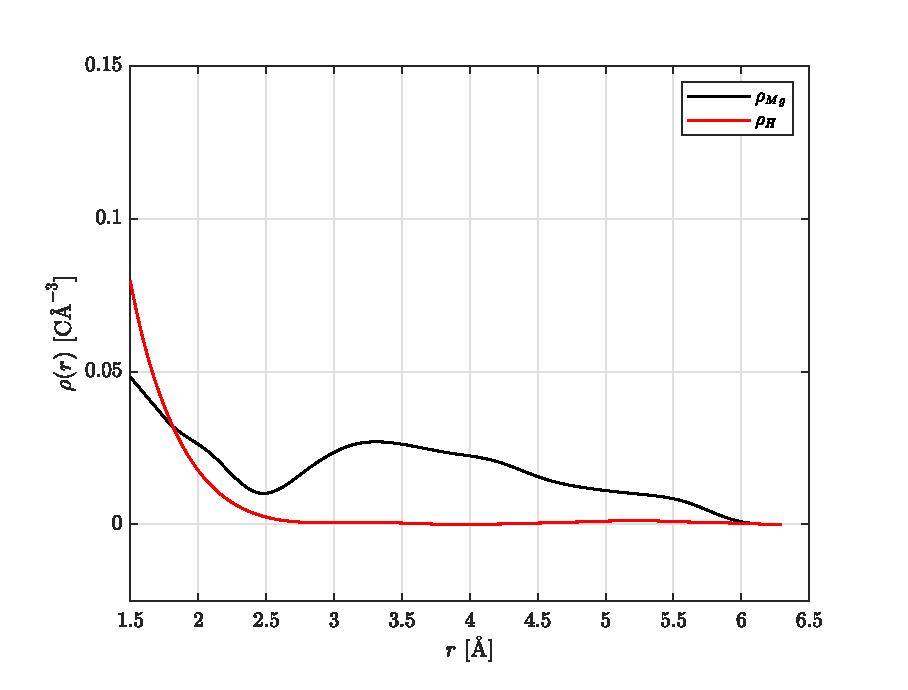
\includegraphics[width=\textwidth]{Figures/rho_MgH.eps}
	\includegraphics[width=\textwidth]{Figures/Fig-Energy-Density.png}
	\caption{Electronic density function $\rho(r)$ for each element}
\end{figure}

\begin{figure}[h!]
	\centering
	%\includegraphics[width=\textwidth]{Figures/phi_MgH.eps}
	\includegraphics[width=\textwidth]{Figures/Fig-Pairing-Function.png}
	\caption{Pair interaction function $\phi(r)$ for each element pair}
\end{figure}

\begin{figure}[h!]
	\centering
	%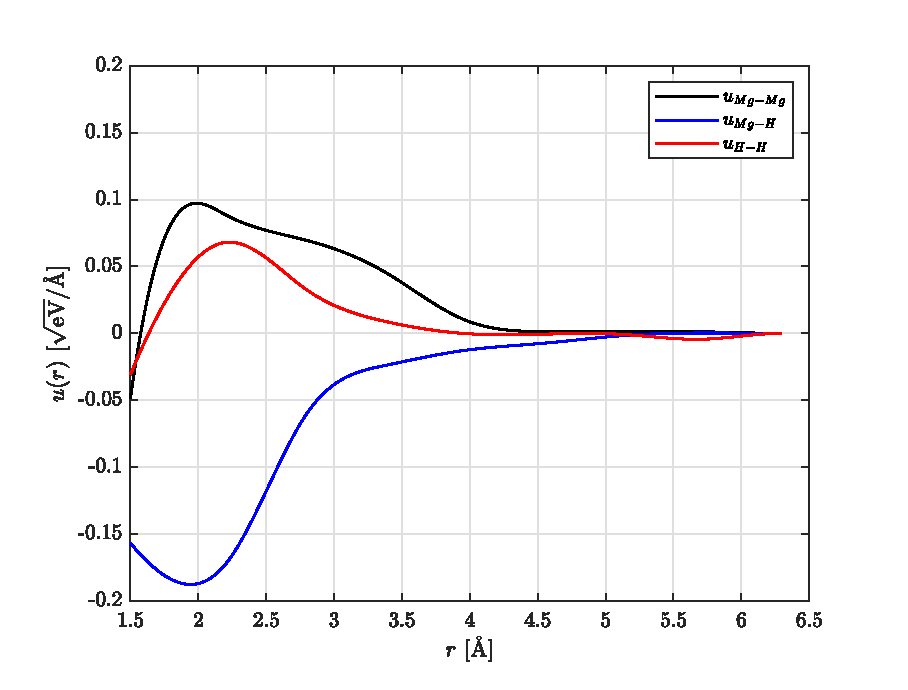
\includegraphics[width=\textwidth]{Figures/u_MgH.eps}
	\includegraphics[width=\textwidth]{Figures/Fig-Dipole-Function.png}
	\caption{Function $u(r)$ for each element pair}
\end{figure}

\begin{figure}[h!]
	\centering
	%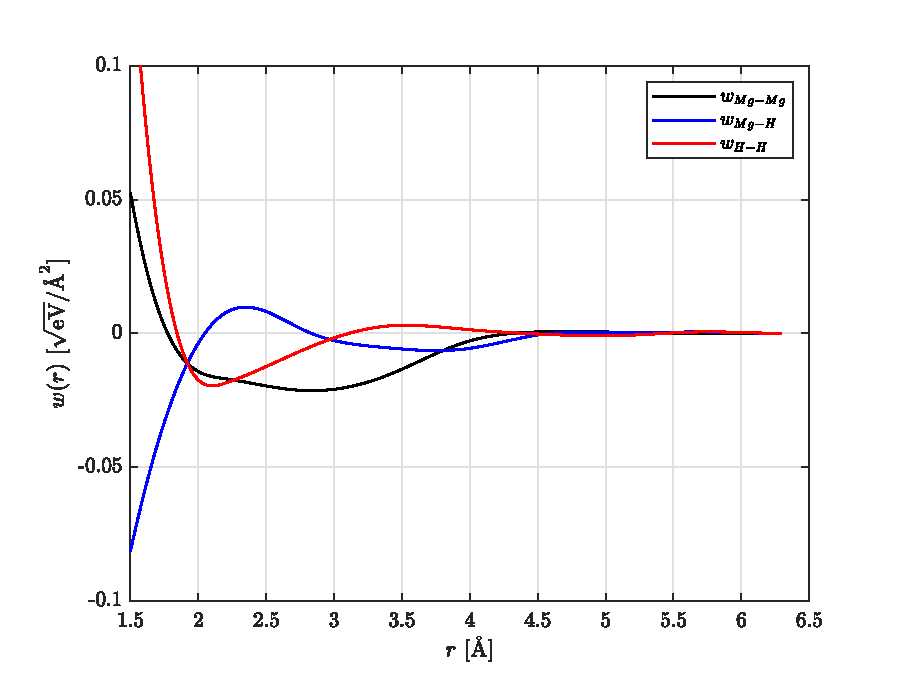
\includegraphics[width=\textwidth]{Figures/w_MgH.eps}
	\includegraphics[width=\textwidth]{Figures/Fig-Quadrupole-Function.png}
	\caption{Function $w(r)$ for each element pair}
\end{figure}

 
\vspace{30cm}

\text{                           }

\newpage


\section{Case of the Al-Cu system}

For the Al-Cu system, the ADP file that we find in the IPR is called \textit{``AlCu.adp''} and its format is the following:

%%%%%%%%%%%%%%%%%%%%%%%%%%%%%%%%%%%%%%%%%%%%%%%%%%%%%%%%%%%%%%%%%
%%%%%%%%%%%%%%%%%%%%%%%%%%%%%%%%%%%%%%%%%%%%%%%%%%%%%%%%%%%%%%%%%
%\begin{comment}
	\setlist[enumerate]{label*=\arabic*.}
	\begin{enumerate}
		\item Header:
		\lstdefinestyle{mystyle}{
			backgroundcolor=\color{backcolour},   
			commentstyle=\color{codegreen},
			keywordstyle=\color{black},
			numberstyle=\tiny\color{codegray},
			stringstyle=\color{codepurple},
			basicstyle=\ttfamily\scriptsize,
			breakatwhitespace=false,         
			breaklines=true,                 
			captionpos=b,                    
			keepspaces=true,                 
			numbers=left,                    
			numbersep=2pt,                  
			showspaces=false,                
			showstringspaces=false,
			showtabs=false,                  
			tabsize=1,
			xleftmargin=10pt,
			xrightmargin=5pt,
			fontadjust=true
		}
		\lstset{style=mystyle}
		%\lstinputlisting[language=Matlab,linerange={1-5},consecutivenumbers=false]{AlCu.adp}
		\item  Sections for the embedding function $F(\rho)$ and the atomic electron density $\rho(r)$ of the $N=2$ elements:
		
		
		\begin{enumerate}
			\item Section of the Al (element 1):
			
			First line:
			%\lstinputlisting[language=Matlab,linerange={6},consecutivenumbers=false]{AlCu.adp}
			
			Block of $N_{\rho}=10000$ values corresponding to the embedding function $F(\rho)$ for Al:
			%\lstinputlisting[language=Matlab,linerange={7-9,10004-10006},consecutivenumbers=false,]{AlCu.adp}
			
			Block of $N_{r}=10000$ values corresponding to the atomic electron density $\rho(r)$ for Al:
			%\lstinputlisting[language=Matlab,linerange={10007-10009,20004-20006},consecutivenumbers=false]{AlCu.adp}
			
			\item Section of the Cu (element 2):
			
			First line:
			%\lstinputlisting[language=Matlab,linerange={20007},consecutivenumbers=false]{AlCu.adp}
			
			Block of $N_{\rho}=10000$ values corresponding to the embedding function $F(\rho)$ for Cu:
			%\lstinputlisting[language=Matlab,linerange={20008-20010,30005-30007},consecutivenumbers=false]{AlCu.adp}
			
			Block of $N_{r}=10000$ values corresponding to the atomic electron density $\rho(r)$ for Cu:
			%\lstinputlisting[language=Matlab,linerange={30008-30010,40005-40007},consecutivenumbers=false]{AlCu.adp}
		\end{enumerate}
		
		\item  Block of $N_rN(N+1)/2=30000$ values corresponding to the scaled pair potential functions $r\phi_{(i,j)}(r)$:
		\begin{enumerate}
			\item Block of $N_r=10000$ values corresponding to the scaled pair potential function $r\phi_{(Al,Al)}(r)$:
			%\lstinputlisting[language=Matlab,linerange={40008-40010,50005-50007},consecutivenumbers=false]{AlCu.adp}
			
			\item Block of $N_r=10000$ values corresponding to the scaled pair potential function $r\phi_{(Al,Cu)}(r)$:
			%\lstinputlisting[language=Matlab,linerange={50008-50010,60005-60007},consecutivenumbers=false]{AlCu.adp}
			
			\item Block of $N_r=10000$ values corresponding to the scaled pair potential function $r\phi_{(Cu,Cu)}(r)$:
			%\lstinputlisting[language=Matlab,linerange={60008-60010,70005-70007},consecutivenumbers=false]{AlCu.adp}
		\end{enumerate}
		
		\item  Block of $N_rN(N+1)/2=30000$ values corresponding to the functions $u_{(i,j)}(r)$:
		\begin{enumerate}
			\item Block of $N_r=10000$ values corresponding to the function $u_{(Al,Al)}(r)$:
			%\lstinputlisting[language=Matlab,linerange={70008-70010,80005-80007},consecutivenumbers=false]{AlCu.adp}
			
			\item Block of $N_r=10000$ values corresponding to the function $u_{(Al,Cu)}(r)$:
			%\lstinputlisting[language=Matlab,linerange={80008-80010,90005-90007},consecutivenumbers=false]{AlCu.adp}
			
			\item Block of $N_r=10000$ values corresponding to the function $u_{(Cu,Cu)}(r)$:
			%\lstinputlisting[language=Matlab,linerange={90008-90010,100005-100007},consecutivenumbers=false]{AlCu.adp}
		\end{enumerate}
		
		
		\item  Block of $N_rN(N+1)/2=30000$ values corresponding to the functions $w_{(i,j)}(r)$:
		\begin{enumerate}
			\item Block of $N_r=10000$ values corresponding to the function $w_{(Al,Al)}(r)$:
			%\lstinputlisting[language=Matlab,linerange={100008-100010,110005-110007},consecutivenumbers=false]{AlCu.adp}
			
			\item Block of $N_r=10000$ values corresponding to the function $w_{(Al,Cu)}(r)$:
			%\lstinputlisting[language=Matlab,linerange={110008-110010,120005-120007},consecutivenumbers=false]{AlCu.adp}
			
			\item Block of $N_r=10000$ values corresponding to the function $w_{(Cu,Cu)}(r)$:
			%\lstinputlisting[language=Matlab,linerange={120008-120010,130005-130007},consecutivenumbers=false]{AlCu.adp}
		\end{enumerate}
	\end{enumerate}
%\end{comment}
%%%%%%%%%%%%%%%%%%%%%%%%%%%%%%%%%%%%%%%%%%%%%%%%%%%%%%%%%%%%%%%%%
%%%%%%%%%%%%%%%%%%%%%%%%%%%%%%%%%%%%%%%%%%%%%%%%%%%%%%%%%%%%%%%%%

Next, the output files for the Al-Cu system created by the script \textit{adp.cpp} are represented.


\begin{figure}[h!]
	\centering
	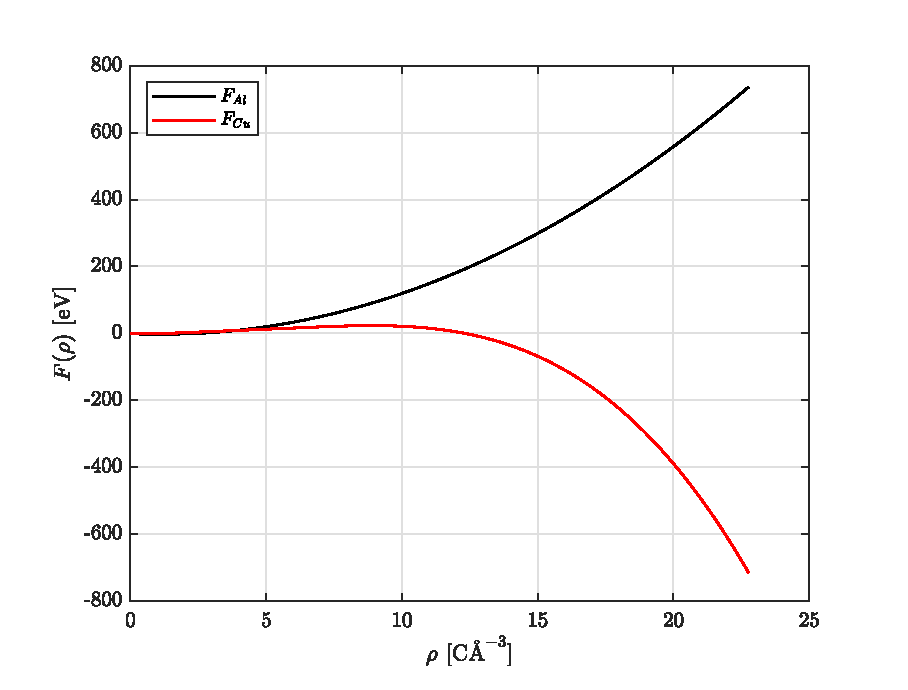
\includegraphics[scale=0.6]{Figures/F_AlCu.eps}
	\caption{Embedding function $F(\rho)$ for each element}
\end{figure}
\begin{figure}[h!]
	\centering
	\includegraphics[scale=0.6]{Figures/rho_AlCu.eps}
	\caption{Electronic density function $\rho(r)$ for each element}
\end{figure}

\begin{figure}[h!]
	\centering
	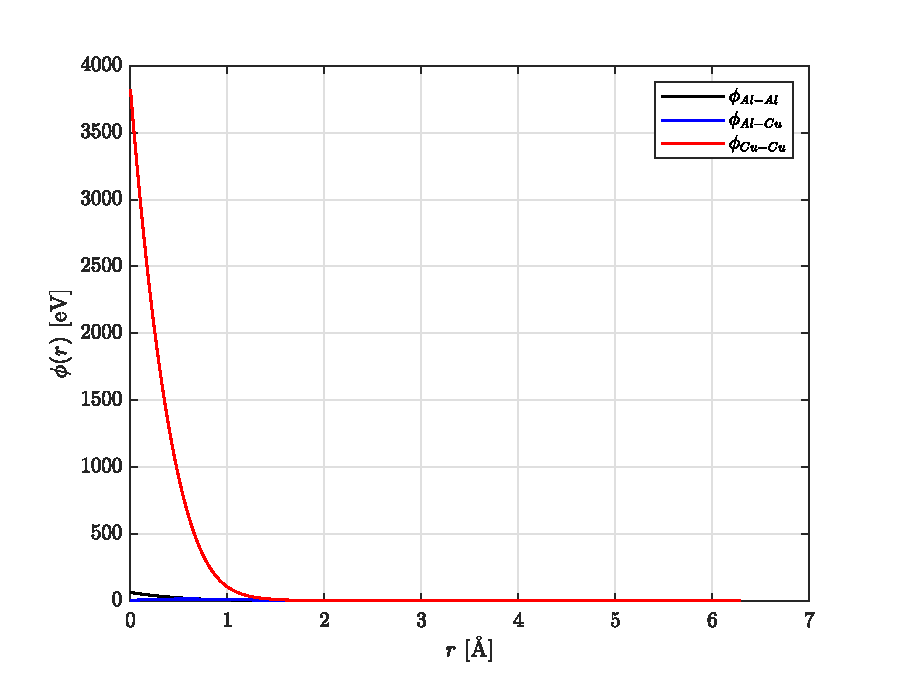
\includegraphics[scale=0.6]{Figures/phi_AlCu.eps}
	\caption{Pair interaction function $\phi(r)$ for each element pair}
\end{figure}

\begin{figure}[h!]
	\centering
	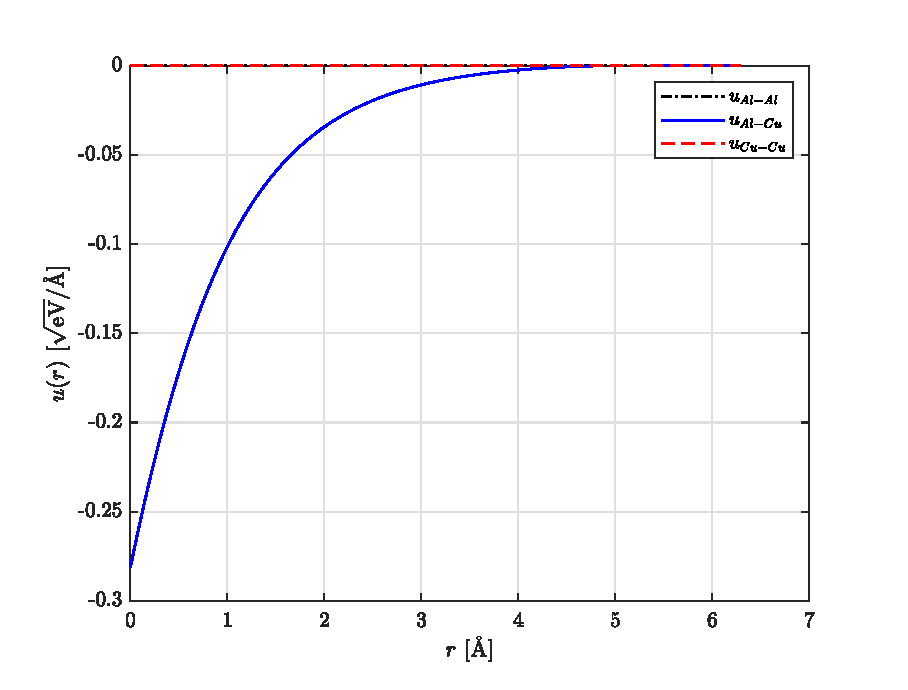
\includegraphics[scale=0.6]{Figures/u_AlCu.eps}
	\caption{Function $u(r)$ for each element pair}
\end{figure}

\begin{figure}[h!]
	\centering
	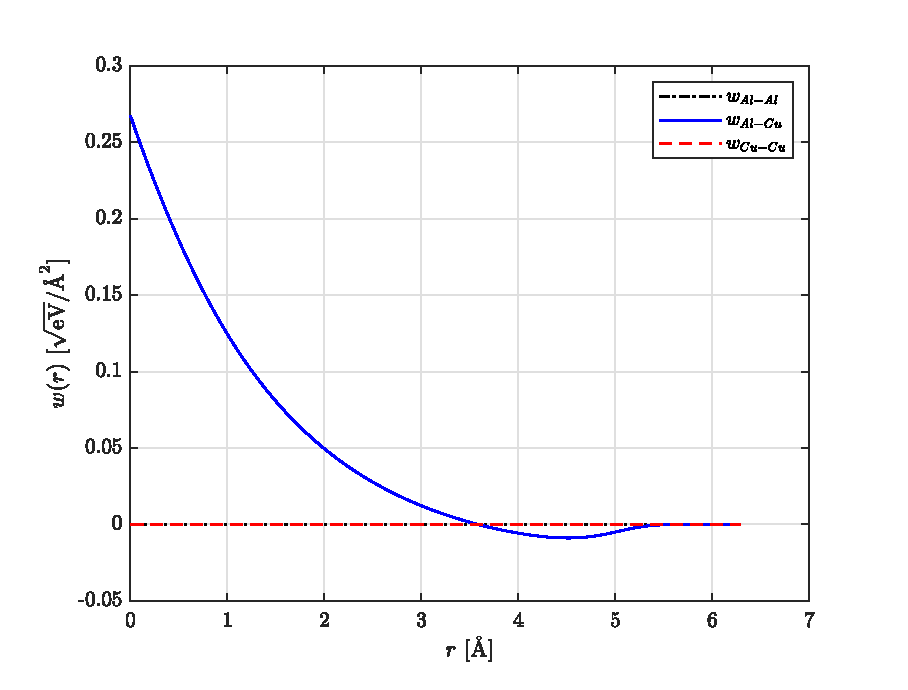
\includegraphics[scale=0.6]{Figures/w_AlCu.eps}
	\caption{Function $w(r)$ for each element pair}
\end{figure}


\vspace{30cm}

\text{                           }

\newpage



\bibliographystyle{plain}
\bibliography{bibliography} 








 
 
\end{document}







